\section{Mitigating Naïve Loss Minimization Leads to Grokking}
\label{sec:avoiding_nmm}

While we have shown in \cref{sec:floating_points} that avoiding numerical instabilities eventually leads to generalization, we can also target the \nlm  process that causes these numerical issues. To do this, we design an optimizer that only preserves the part of the gradient orthogonal to the direction of the weights.

\subsection{$\ograd$: An optimizer to prevent NLM}

\begin{figure*}[t]
\begin{subfigure}[t]{.32\textwidth}
    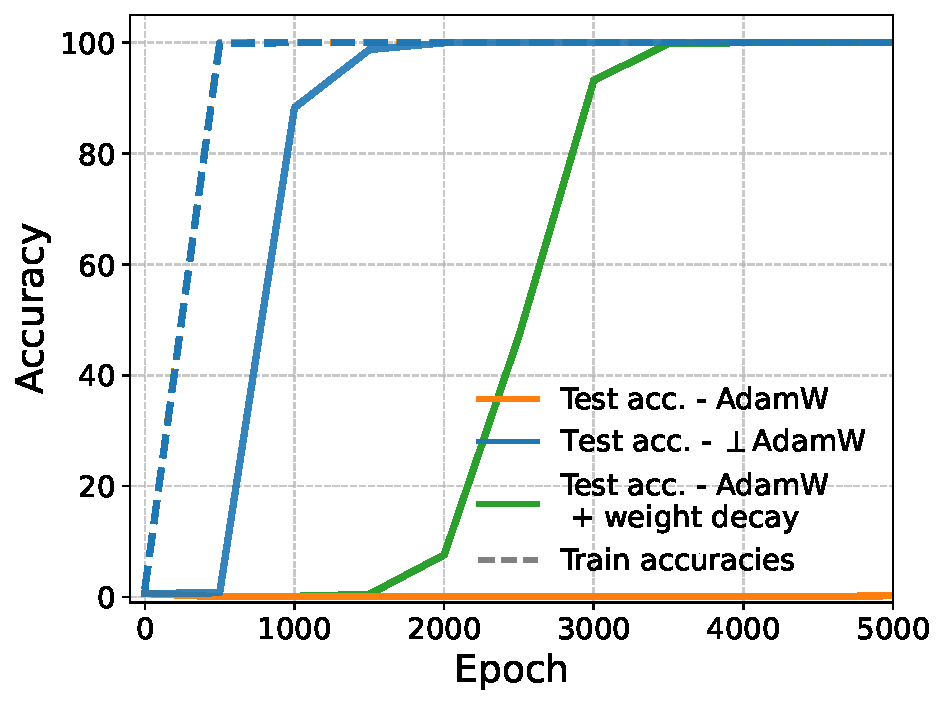
\includegraphics[width=\linewidth]{grokking_iclr_arxiv/figures/transformer_orthogonal.pdf}
    \caption{\vspace{-1.5mm}Transformer, subtract. mod 113}
    \label{fig:orthogonal_gradient}
\end{subfigure}
\hfill
\begin{subfigure}[t]{.32\textwidth}
    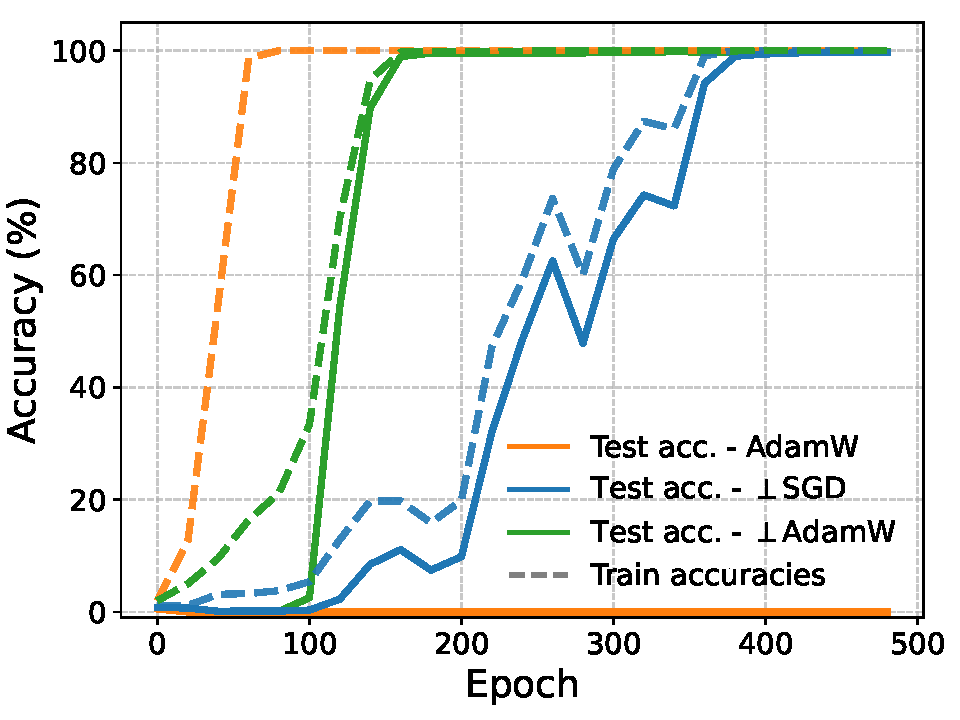
\includegraphics[width=\linewidth]{grokking_iclr_arxiv/figures/mlp_orth_gradients.pdf}
    \caption{\vspace{-1.5mm}MLP, addition mod 113}
\label{fig:orthogonal_gradient_mlp}
\end{subfigure}
\hfill
\begin{subfigure}[t]{.32\textwidth}
  \centering
  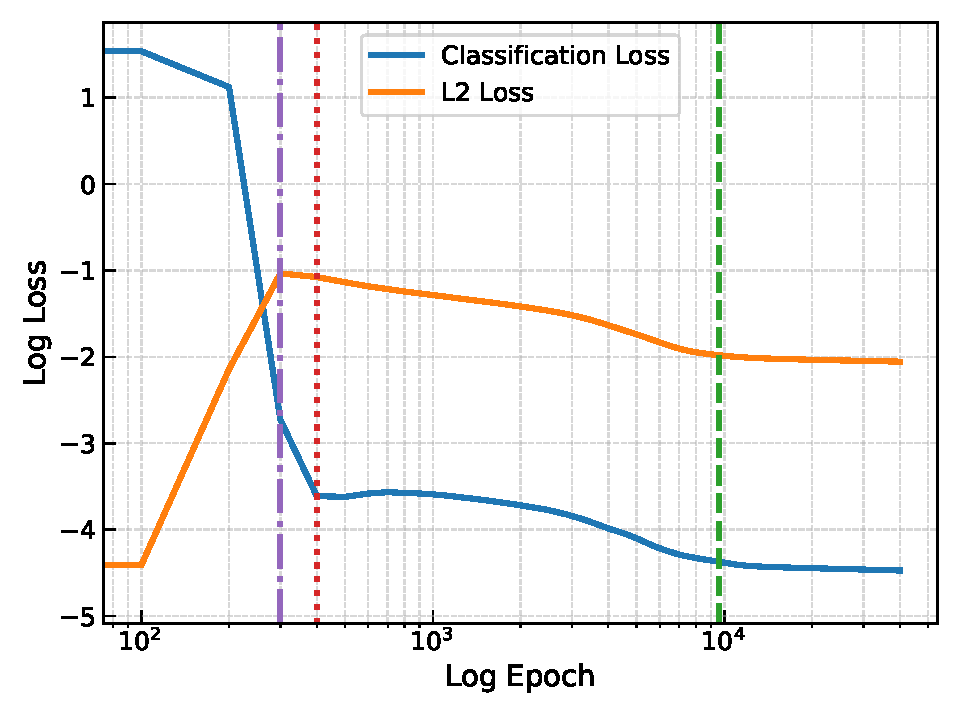
\includegraphics[width=\linewidth]{grokking_iclr_arxiv/figures/l2_v_classification_loss.pdf}
  \caption{\vspace{-1.5mm}Trade-off between L2 and SCE}
  \label{fig:l2_vs_sce}
\end{subfigure}
\vspace{-1mm}
\caption{Comparing $\perp$AdamW and $\perp$SGD with baseline optimizers and AdamW with weight decay on (\textbf{a}) a transformer trained on subtraction mod 113 and  (\textbf{b}) an MLP trained on addition modulo 113. In (\textbf{c}) we highlight the trade-off between L2 regularization and SCE loss, initially SCE loss is reduced at the cost of increasing the L2 loss but eventually the two losses decrease simultaneously (\cref{sec:explain_existing_methods}). \vspace{-7mm}}
\end{figure*}

We propose a new optimizer, $\perp$\textbf{Grad} (read ``ortho-grad''), that updates the weights based only on the part of the gradient that is orthogonal to the current direction of the weights:

\begin{dfn}[$\perp$Grad]
    We propose the following update rule for a given iteration $t \in \mathbb{N}$: 
    \begin{equation}
        \bm{\theta}_{t+1} = \bm{\theta}_t - \eta \nabla_{\perp} \loss(\bm{\theta}_t),
    \end{equation}
    where the orthogonal component 
 of the gradient, $\nabla_{\perp} \loss(\bm{\theta}_t)$, is obtained by projection onto the hyperplane orthogonal to the current weight vector: 
 \begin{equation}
     \nabla_{\perp} \loss(\bm{\theta}_t) = \nabla \loss(\bm{\theta}_t) - \left( \frac{\bm{\theta}_t^\top \nabla \loss(\bm{\theta}_t)}{\bm{\theta}_t^\top \bm{\theta}_t} \right) \bm{\theta}_t.
 \end{equation}
%NMMGrad converges since $\nabla_{\perp} \loss(\bm{\theta}_t)$ is a descent direction.
\end{dfn}
\begin{prop}\label{prop:NLMGrad}
    Assuming $\nabla_{\perp} \loss(\bm{\theta}_t)\neq \mathbf{0}$, $\exists~\beta>0$ such
that for any learning rate $0 <\eta<\beta$, taking the step $\eta\nabla_{\perp} \loss(\bm{\theta}_t)$ reduces the loss. In other words, any nonzero $\nabla_{\perp} \loss(\bm{\theta}_t)$ is a descent direction.
\end{prop}
\vspace{-7pt}
\begin{proof}[Sketch of the proof.]
We show that any $\nabla_{\perp} \loss(\bm{\theta}_t) \in \mathbb{R}^m\backslash\{\mathbf{0}\}$ is a descent direction by demonstrating that $\left\langle -\nabla_{\perp} \loss(\bm{\theta}_t), \nabla\loss(\bm{\theta}_t) \right\rangle < 0$. For a full proof we refer the reader to~\cref{app:proofs}.
\end{proof}

This projection of the gradient can be incorporated into different optimizers. In \cref{fig:orthogonal_gradient}, we show results for $\perp$AdamW and $\perp$SGD, the $\perp$Grad versions of AdamW and SGD respectively. These results show that $\perp$Grad optimizers lead to generalization without a phase of initial overfitting, in contexts where no improvement in test performance is usually observed without weight decay. We note that similar projections of the gradients have been used in other settings to mitigate the effects of momentum in invariant layers \citep{adamp2020}, stabilize training \cite{wang2024achieving} or as one part in a more complex optimizer \citep{kosson2024rotational}. We design \ograd as a more precise intervention that direcly prevents scaling along the NLM direction.

In~\cref{fig:loss_landscape}, we compare the trajectories of models using SGD with and without weight decay to our new $\perp$SGD optimizer. SGD models start on a similar trajectory, reducing the training loss but increasing the test loss, until the model with weight decay changes direction and starts minimizing both the train and test loss. In contrast, the model using $\perp$SGD moves directly in a direction that minimizes both the train and test loss. While SGD with weight decay eventually reaches a point of lower loss, note that $\perp$SGD reaches 100\% test accuracy within 400 iterations (\cref{fig:orthogonal_gradient}). Beyond showing how $\perp$SGD prevents NLM, \cref{fig:loss_landscape} also suggests that weight decay induces grokking by avoiding NLM. In the following, we highlight that the success of several methods to induce grokking can be explained from this perspective.


\begin{figure}[t]
\begin{subfigure}[t]{.48\textwidth}
    \centering
    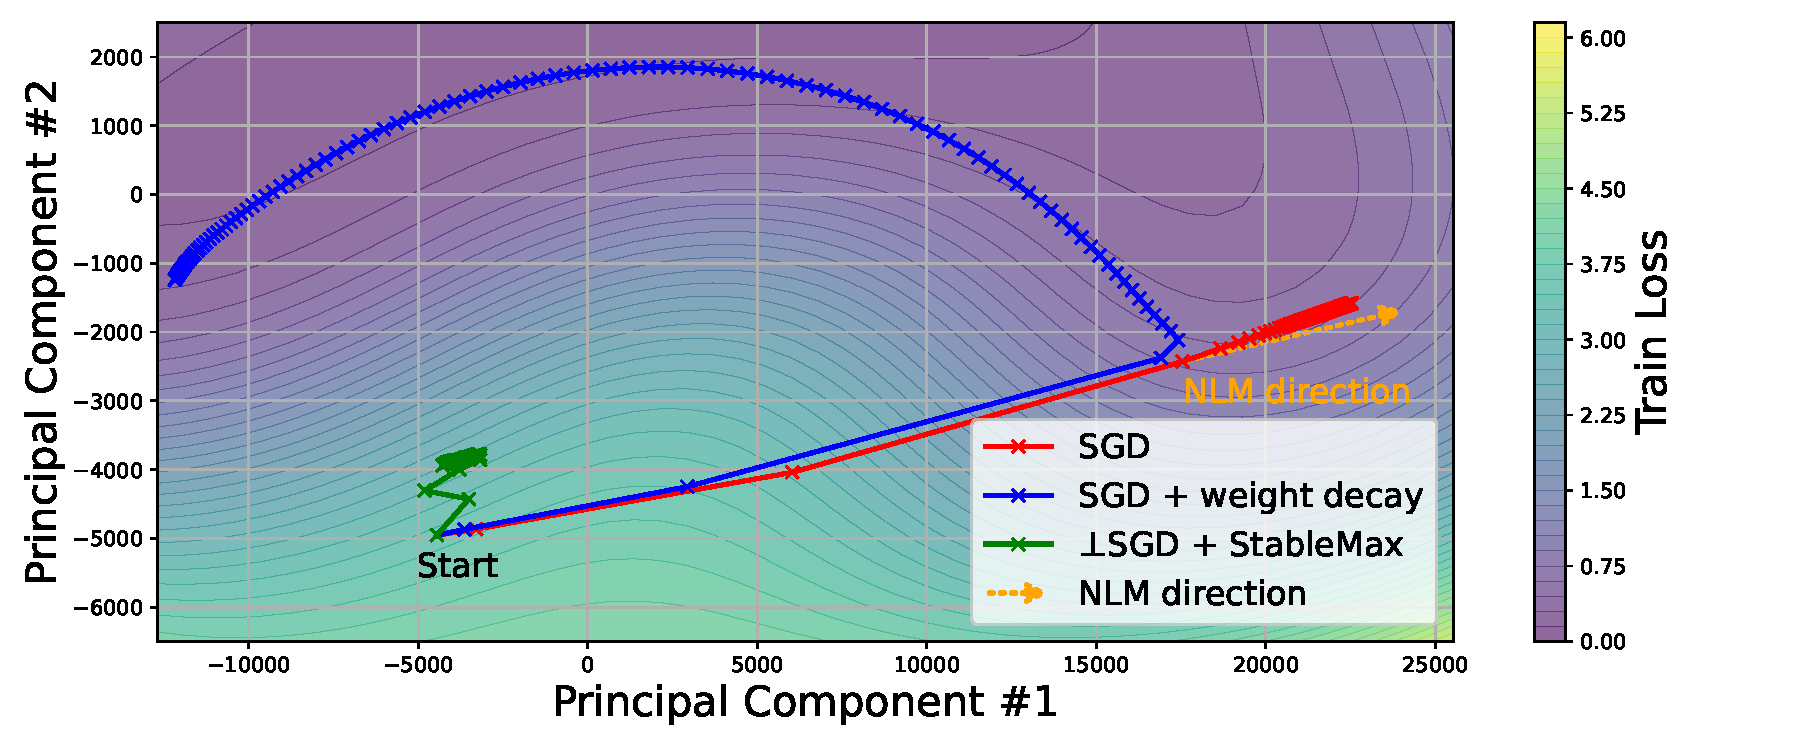
\includegraphics[width=\linewidth]{grokking_iclr_arxiv/figures/trajectory_with_loss_landscape_train.pdf}
    \caption{Training loss landscape}
    \label{fig:trajectory_plot}
\end{subfigure}
\hfill
\begin{subfigure}[t]{.48\textwidth}
  \centering
  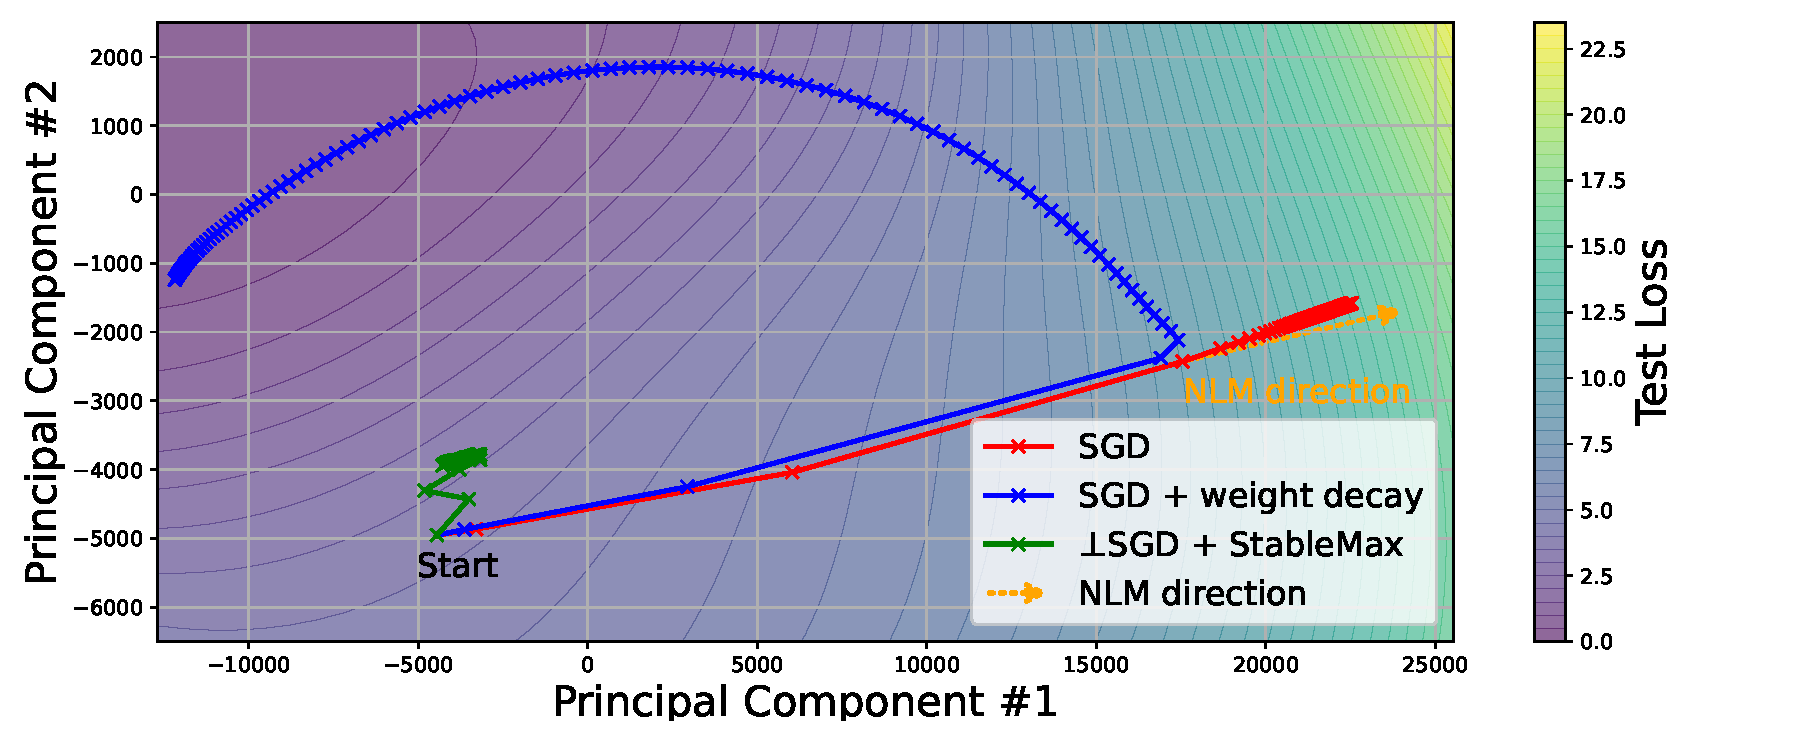
\includegraphics[width=\linewidth]{grokking_iclr_arxiv/figures/trajectory_with_loss_landscape_test.pdf}
  \caption{Test loss landscape}
\end{subfigure}
\vspace{-3mm}
\caption{Model trajectories in in parameter space projected to 2D over the SCE loss landscape. SGD with weight decay starts along the same trajectory as SGD decreasing the training loss \textbf{(a)} but increasing the test loss \textbf{(b)}.\vspace{-6 mm}}
\label{fig:loss_landscape}
\end{figure}
% Eventually, the test loss starts to decrease for the model with weight decay while SGD without weight decay continues along NLM direction. The NLM direction is highlighted as the direction that corresponds to scaling up all the weights by 20\% for the first model to reach 100\% train accuracy with SGD. Note that the "detour" taken by the model with weight decay corresponds to the delay in generalization observed during grokking and that $\perp$SGD decreases the test loss from the beginning, without a delay in generalization
\subsection{Explaining the success of existing methods for grokking}\label{sec:explain_existing_methods}

In light of our findings, we are able to explain the success of several previously proposed methods to induce grokking. We find that these methods also lead to grokking by mitigating NLM and avoiding the FP errors that come with extremely low losses.

\paragraph{Weight decay} We have argued that the problem faced in grokking is that the ease of overfitting leads to \nlm, which corresponds to scaling up the weights for homogeneous networks. Since weight decay corresponds to pulling back the weights along this same direction at every step during training, it is unsurprising, given our findings, that it is the most reliable way to induce grokking. 

To explain why generalization tends to be delayed when using weight decay, as opposed to $\perp$Grad, we look at it from the perspective of L2 regularization which is equivalent to weight decay for SGD. In~\cref{fig:l2_vs_sce}, we see an initial phase where classification loss decreases, at the cost of the L2 loss.  Eventually, the decrease in classification loss from \nlm stops outweighing the increase in L2 loss, meaning that only updates that are not aligned with the NLM direction are followed. This explains why weight decay leads to generalization in grokking tasks but only after scaling along the \nlm direction no longer decreases the overall loss. This balance between weight decay and classification loss is similar to the rotational equilibrium studied in \cite{kosson2024rotational}.

We argue that the main roles of weight decay are preventing floating point errors and preventing NLM. This is in line with recent findings about the role of weight decay in deep learning \citep{andriushchenko2023needweightdecaymodern} which point to the fact that it increases the effective learning rate and avoids floating point issues when using mixed-precision training in LLMs.

\paragraph{MSE loss on shallow networks}
While cross-entropy loss can be reduced indefinitely by scaling the logits through \nlm, this is not the case with MSE loss. When using MSE loss the logits can overshoot the target, meaning that larger logits often do not lead to a lower MSE loss. This explains why \cite{Barak2022-el}, \cite{Kumar2023-hz}, and \cite{Lyu2023-ga} observed grokking with MSE loss without regularization. Interestingly, networks with more than one hidden layer do not generalize in these same settings (\cref{fig:alpha_parameter}).

\paragraph{Delaying generalization by scaling the weights}
While the lazy training dynamics described in \cite{Kumar2023-hz} explain an important part of why scaling the weights delays generalization, we show that the reason that regularization is often needed to exit this lazy training regime is that scaling the weights or the logits facilitates SC.  In \cref{app:scaling_weights}, we show that the setting used in \cite{liu2023grokking} to induce grokking on MNIST with SCE also induces SC which prevents further learning in the absence of weight decay.